\section{Introduction}
\label{sec:introduction}

Loop Engineering marks a shift in how developers interact with coding agents on long-running tasks.
Instead of inspecting each result and writing the next prompt by hand, developers specify the task goal and the criteria for judging progress, then let a loop manage the successive rounds of interaction \citep{Osmani2026LoopEng}.
LoopArena evaluates a model's ability to manage these rounds through a two-agent harness: the evaluated model is the \textbf{Controller}, while a separate \textbf{Worker} carries out the coding task.
We refer to the Worker's task execution as the \textbf{inner loop} and the Controller's guidance of the overall process as the \textbf{outer loop}.
Figure~\ref{fig:runtime} shows how the Controller's outer loop guides the Worker's inner loop.

Once a coding agent works across many steps, a plausible partial result can easily be mistaken for completion: a narrow check may pass while another requirement remains untouched. As the repository and available evidence evolve, the next useful instruction may shift from implementation to verification, recovery, or stopping.
LoopArena evaluates whether a Controller can recognize such situations, redirect the Worker when necessary, and decide when the run should end.
In the \textbf{Controller-guided} condition, the Controller reviews the run after each Worker round and decides how the next round should proceed.
We also report a \textbf{no-control} baseline in which the same Worker receives the task instruction and works autonomously to completion.
We additionally evaluate \textbf{fixed control}, a persistent-goal baseline inspired by Codex's \texttt{/goal}: at every control point, the harness deterministically restates the original task objective and asks the Worker to continue, without adapting its guidance to the current evidence.

\begin{figure}[t]
\centering
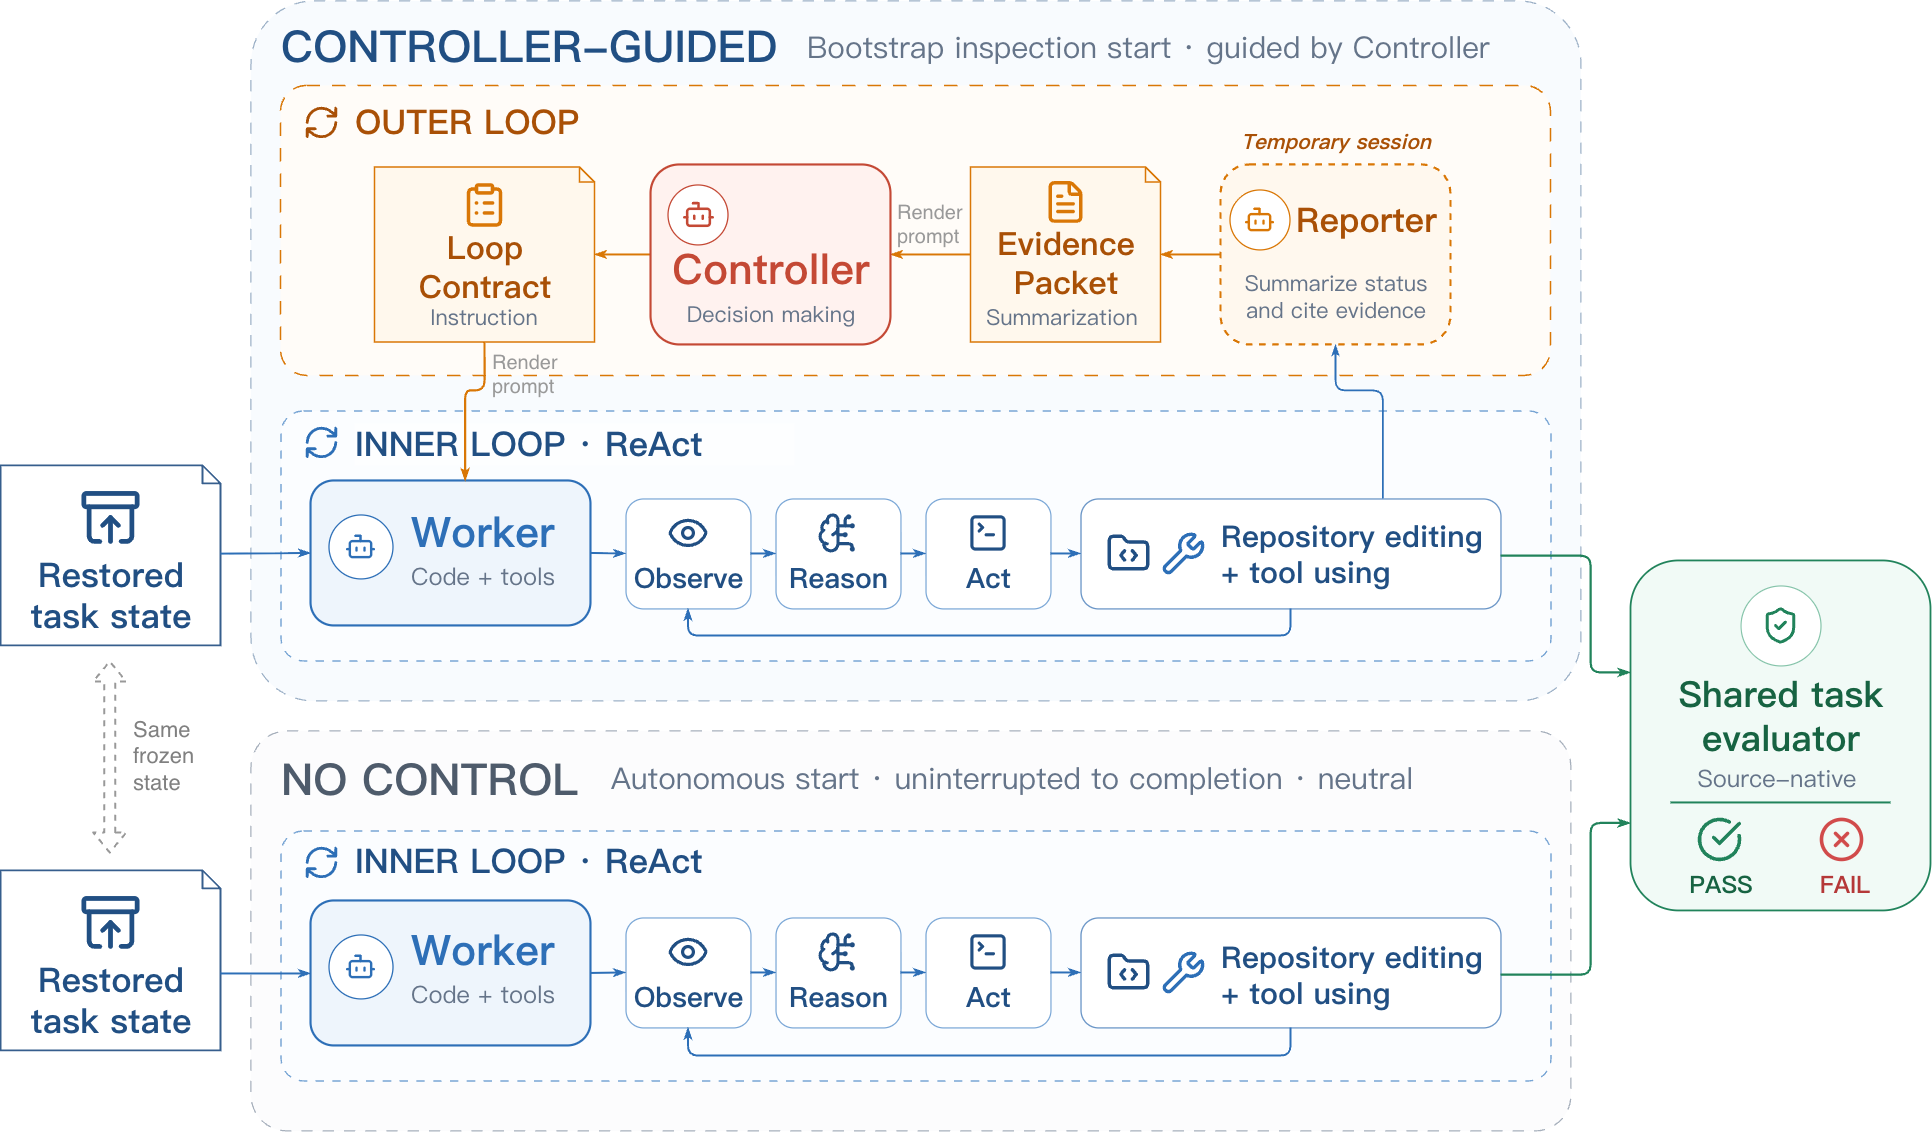
\includegraphics[width=0.98\linewidth]{looparena_harness.png}
\caption{\textbf{The LoopArena harness.} Both conditions start from the same restored task state and use the same Worker, coding tools, and task evaluator. In the Controller-guided condition, a temporary \textbf{Reporter} agent summarizes the Worker's progress after each round, and the harness deterministically formats the report as an \textbf{Evidence Packet}. The Controller reads this structured, read-only summary and issues a \textbf{Loop Contract} specifying the next Worker segment, or decides to stop. In the no-control condition, the Worker runs without Controller guidance.}
\label{fig:runtime}
\end{figure}

Most coding benchmarks \citep{Jimenez2023,MultiSWEBench2025} evaluate task completion by running a coding agent and scoring the resulting repository state with executable tests or task-specific evaluators.
Long-horizon and iterative benchmarks extend this setup to longer tasks or evolving requirements, but still score the coding agent or agent system as a whole \citep{SlopCodeBench}.
Process-oriented benchmarks instead assess individual actions or capabilities within the coding trajectory, such as repository exploration \citep{AgentProcessBench2026,SWEExplore2026}.
Recent work has begun to benchmark different combinations of coding models and loop implementations on long-horizon tasks \citep{LoopsBench2026}.
LoopArena targets a different object of evaluation: a model's ability to control the loop around a separate coding agent.
This model-as-manager setting makes agent orchestration directly evaluable: the Controller interprets the ongoing run and decides what the Worker should do next.

To evaluate this ability, we compare models in the Controller role while keeping the Worker and execution setup fixed. Each time the Worker returns control to the harness after working on its current assignment, the harness creates a temporary \textbf{Reporter} agent using the same model as the Worker and a copy of the Worker conversation history. The Reporter summarizes the current state of the task from this history and read-only workspace inspection. It runs in a temporary copy of the conversation, so its interaction does not alter the persistent Worker history. The harness deterministically formats the Reporter's summary and the Worker's working evidence it cites into an \textbf{Evidence Packet}, which is a structured, read-only summary for the Controller. The Controller reads this Packet and issues a structured \textbf{Loop Contract} that either specifies the Worker's next assignment or ends the run. If work continues, the harness converts the Contract into the Worker's next prompt. The Controller has no coding tools and can affect the task only through the instructions it sends to the Worker.

LoopArena organizes evaluation into three complementary settings that differ in execution scope and cost. \textbf{Type III} evaluates Controller models on complete, long-horizon repository-level coding tasks, beginning from the original task specification and repository state. \textbf{Type II} evaluates runtime loop control on one selected task slice from the same full task. In our experiments, the paired Type II cost reduction averages \textbf{60.6\%} across Controllers, and its ordering is positively correlated with Type III under the main Core criterion (Spearman's correlation \(\rho=\textbf{0.7353}\)). \textbf{Type I} moves its execution cost to benchmark construction. During construction, we execute candidate Loop Contracts and use their downstream outcomes to establish the correct option; once the benchmark is built, each new Controller is scored through a single four-way choice with no Worker execution. Together, the three settings support low-cost diagnosis of individual control decisions, lower-cost evaluation of runtime loop control, and end-to-end evaluation on long-horizon coding tasks.

Our contributions are the following:
\begin{enumerate}

\item \textbf{A benchmark for runtime loop control.}
LoopArena evaluates how well a model decides what a separate coding agent should do next and guides it through long-horizon repository-level tasks, making runtime loop control a direct target of evaluation.

\item \textbf{A controlled protocol for comparing Controller models.}
Across Controller-model comparisons, LoopArena holds the Worker and execution setup fixed, including the tools, task environment, execution budget, evaluator, and control interface. The object of comparison is therefore the Controller model, not the complete coding-agent system.

\item \textbf{Evaluation at decision, task-slice, and full-task levels.}
Type I shifts candidate execution to benchmark construction, enabling low-cost control questions grounded in downstream outcomes. Type II and Type III evaluate runtime loop control on paired task slices and full tasks. This pairing lets us quantify the reduction in evaluation cost and compare Controller rankings across the two execution scopes.

\end{enumerate}

\section{The LoopArena Benchmark}
\label{sec:benchmark}

\subsection{Evaluation tasks}
\label{sec:evaluation-tasks}

LoopArena evaluates Controller ability at three levels of execution scope and evaluation cost: a single control decision in Type I, a task slice in Type II, and the corresponding full task in Type III.

\paragraph{Type I: Contract selection.} Type I evaluates a single control decision. At one control point, the Controller receives an Evidence Packet and chooses among four candidate Loop Contracts for the next Worker round. The execution needed to determine the correct option is completed in advance as part of benchmark construction. Evaluating a new Controller therefore requires only a four-way choice and no Worker execution.

\paragraph{Type II: Condensed coding task.} Type II evaluates one slice of a full coding task. Each case begins from a prepared intermediate workspace in which the preceding work is complete and asks the Controller--Worker loop to complete the next coherent stage. The evaluator checks the cumulative requirements through that stage. Starting partway through the task reduces the execution required for each evaluation.

\paragraph{Type III: Full coding task.} Type III evaluates the corresponding full task from its original state. The Controller manages the complete run, from the Worker's initial investigation through implementation and verification to the final decision to stop. Each Type II case is paired with the full task from which its slice was constructed, allowing direct comparisons of evaluation cost and Controller ordering across the two settings.

\subsection{Control cycle}
\label{sec:control-cycle}

LoopArena maintains a persistent Worker conversation throughout each run. The Worker is the only component that can use coding tools: within each assigned segment, it follows its native ReAct loop to inspect and modify the repository, run checks, and carry out the assigned work \citep{ReAct2022,CodeAct2024}. In the Controller-guided condition, a Loop Contract either defines the next Worker segment or ends the run. When the Worker completes a segment and returns control to the harness, the persistent conversation is paused and a control cycle begins.

At the start of each control cycle, the harness creates a temporary Reporter agent from a copy of the accumulated Worker conversation. The Reporter uses the same model configuration as the Worker and may inspect the workspace only through read-only tools. It produces a four-part account of the run: the task context, the work completed and current state, the available verification evidence, and the remaining issues. Material claims in the report cite the corresponding Worker turns. The Reporter describes the current state but does not decide what should happen next. Its interaction remains separate from the persistent Worker conversation, and it cannot execute code, run tests, or modify the repository.

For executable task \(i\) at control cycle \(k\), the harness packages the report and cited Worker turns into an Evidence Packet \(x_{i,k}\), a structured, read-only summary for the Controller. We denote the Controller model by \(\pi\). Let \(h_{i,k}\) denote its conversation history before this decision, including earlier Packets and Contracts. At each control point, the Controller receives the latest Packet together with this history, but has no direct access to the workspace or coding tools. It produces a Loop Contract \(c_{i,k}\):
\[
c_{i,k}=\pi(x_{i,k},h_{i,k}).
\]
The Contract records the Controller's decision to advance the work, request focused verification, or stop. When the Controller chooses to proceed, the Contract gives the Worker a bounded next assignment and specifies when control should return to the harness. The harness renders this assignment as the next instruction in the persistent Worker conversation. When the Controller chooses to stop, the harness sends the current workspace to the task evaluator. We refer to this sequence as one control cycle. Exact Packet and Contract schemas are given in Appendix~\ref{app:schema}.

\section{Benchmark Construction}
\label{sec:construction}

\begin{figure}[t]
\centering
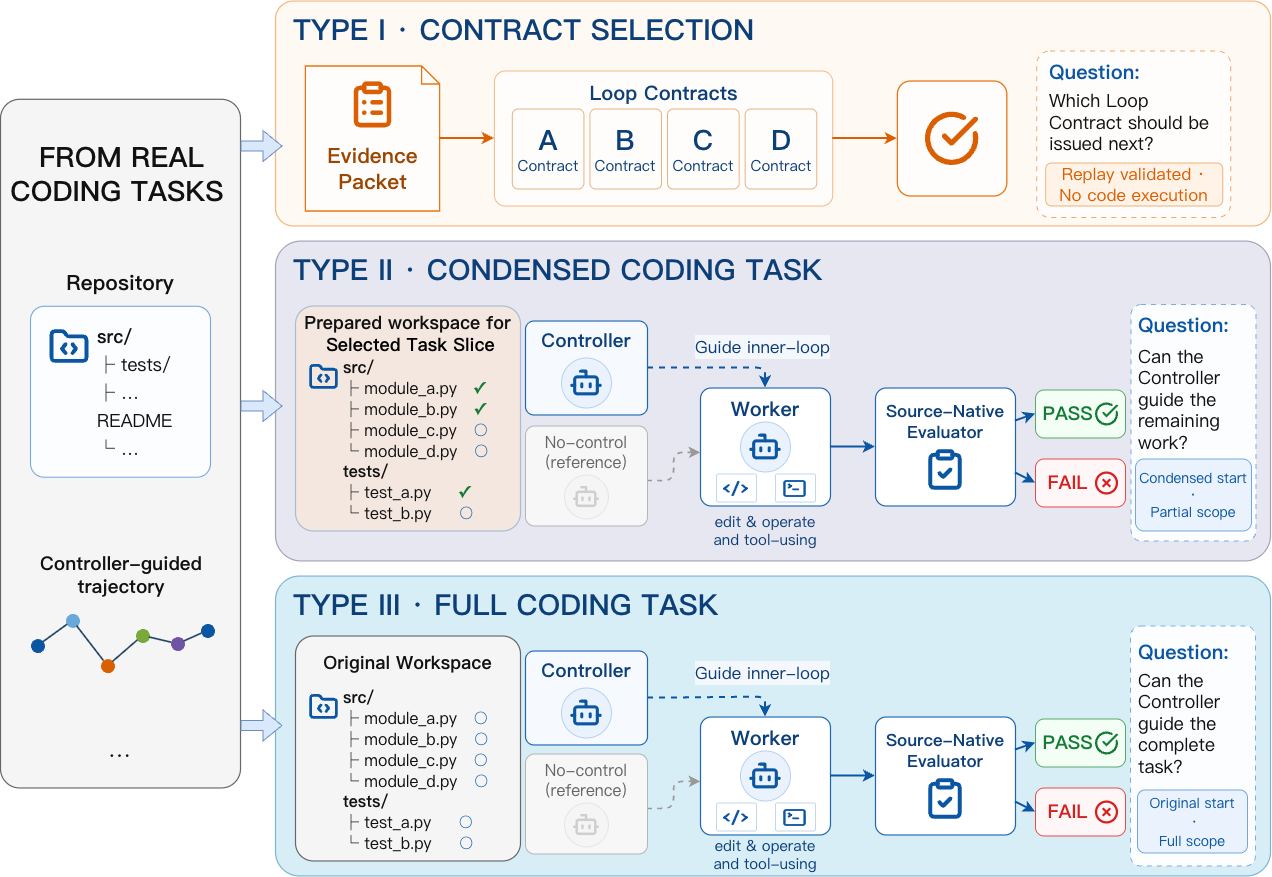
\includegraphics[width=0.98\linewidth]{looparena_task_forms.png}
\caption{\textbf{Constructing the three LoopArena settings.} Type III evaluates a full coding task from its original state. Type II starts from a prepared intermediate workspace and evaluates one slice of the same task. Type I uses a restorable control point from a Controller-guided trajectory and determines the correct option by replaying all four candidate Loop Contracts.}
\label{fig:task-forms}
\end{figure}

LoopArena uses full coding tasks from SlopCodeBench (SCBench) \citep{SlopCodeBench}, BeyondSWE \citep{BeyondSWE2026}, and LoopsBench \citep{LoopsBench2026}. Type III evaluates each task from its original state, while Type II pairs it with one task slice beginning from a prepared intermediate workspace. Type I constructs execution-validated control questions at restorable points in Controller-guided trajectories (Figure~\ref{fig:task-forms}). The construction focuses on tasks, intermediate states, and control decisions where plausible control choices can lead to different executable outcomes.

\subsection{Source tasks and task slices}

The source benchmarks provide complementary task structures: SCBench targets long-horizon iterative coding, BeyondSWE covers software-engineering tasks beyond single-repository bug fixing, and LoopsBench provides long-horizon coding tasks. For Type III, we retain each selected task's original specification, starting state, development process, and evaluator. For Type II, SCBench supplies task slices from its native checkpoints. BeyondSWE tasks are divided into coherent development stages using the official repair and its tests; one stage is selected to form the task slice. LoopsBench likewise pairs each full task with a selected stage and its prepared workspace.

\subsection{Constructing Type II cases}

For each full task, Type II selects one stage that can be evaluated from a prepared intermediate workspace. The case describes the work required for that stage, and its evaluator checks the requirements that should hold when the stage is complete. We retain a slice only when the starting workspace fails at least one requirement introduced by the stage and the source-provided completed state passes all requirements expected at that point. Each Type II case remains paired with its corresponding Type III task for matched comparisons of evaluation cost and Controller ordering. The prepared workspace contains the implementation of earlier stages. Completing the selected stage requires new changes to work with this existing code, and the cumulative evaluator checks both the new requirements and the earlier requirements that remain applicable. Starting from this state saves the preceding execution while retaining the need to extend and verify an existing implementation.

\subsection{Constructing Type I questions}

Type I questions are constructed at restorable control points in Controller-guided trajectories. Each question is anchored immediately before a recorded Controller decision. The Evidence Packet at that point provides the question context. The recorded Loop Contract is retained as one of four candidates, together with three complete alternatives. The four candidates and their presentation order are frozen before any replay outcome is observed.
We execute the four candidates under two predeclared matched replay schedules from the same restored state, holding the Worker, budget, evaluator, continuation policy, and stopping rules fixed. A candidate becomes the correct option only when it is the same unique winner under both schedules according to the ordering specified in Appendix~\ref{app:construction}: task success first, followed by fewer downstream Controller cycles and then fewer Worker turns; items without such a winner are rejected. Once the item is frozen, evaluating a new Controller requires one four-way response and no Worker execution.

\subsection{Benchmark validation}
\label{sec:admission}

Benchmark construction combines source-specific automated checks with LLM-assisted and expert review where semantic judgment is required. We verify task, workspace, and evaluator consistency; enforce the Type II validity conditions above; confirm a stable replay-defined answer for every Type I question; and check that model inputs do not expose solution code, final scoring results, or later events from the source trajectory. Task and slice selection are fixed before formal Controller evaluation. Post-freeze LLM-assisted and expert audits assess Type I clarity and candidate plausibility without changing the replay-defined answers. Appendix~\ref{app:admission} gives the source-specific construction rules and review criteria.
Table~\ref{tab:benchmark-composition} summarizes the three settings.

\begin{table}[t]
\caption{\textbf{Benchmark composition and evaluation statistics.} Type II and Type III use the same \NumTypeIII{} source tasks. Source counts are listed in SCBench/BeyondSWE/LoopsBench order. Bar lengths represent the average Worker turns per run across the evaluated Controllers. The ranges in the final two columns span the corresponding per-Controller means. Type I requires no Worker execution.}
\label{tab:benchmark-composition}
\centering
\small
\setlength{\tabcolsep}{4pt}
\begin{tabular*}{\linewidth}{@{\extracolsep{\fill}}lcclr@{}}
\toprule
& \multicolumn{2}{c}{Instances} & \multicolumn{2}{c}{Per-run statistics} \\
\cmidrule(lr){2-3}\cmidrule(lr){4-5}
Setting & Total & By source & Worker turns & Control cycles \\
\midrule
Type I & \NumTypeI{} & 40 / 53 / 67 & --- & --- \\
Type II & \NumTypeII{} & 21 / 29 / 30 & \raisebox{0.35ex}{\rule{8.0mm}{5pt}}\enspace 86.61--145.30 & 3.55--5.42 \\
Type III & \NumTypeIII{} & 21 / 29 / 30 & \raisebox{0.35ex}{\rule{18.9mm}{5pt}}\enspace 189.41--355.94 & 8.16--13.45 \\
\bottomrule
\end{tabular*}
\end{table}

\section{Evaluation Metrics}
\label{sec:evaluation-metrics}

LoopArena evaluates control at two scales: isolated decisions and their consequences under execution. Type I scores a single Contract choice from a frozen state. Types II and III score repeated control over a task slice and its paired full task. The executable settings also compare inference cost and the Controller orderings obtained at the two execution scopes.

\subsection{Type I: Contract selection}

Each Type I question \(q\) presents the Controller \(\pi\) with a frozen Evidence Packet and four candidate Loop Contracts. The Controller selects one candidate without running the Worker. Let \(j_q^\star\in\{1,2,3,4\}\) be the correct option fixed during benchmark construction, and let \(\widehat{j}_{\pi,q}\in\{1,2,3,4,\bot\}\) be the parsed response, where \(\bot\) denotes an invalid response. Contract Accuracy is
\[
\operatorname{Acc}_{\mathrm{I}}(\pi)
=
\frac{1}{N_{\mathrm{I}}}
\sum_{q=1}^{N_{\mathrm{I}}}
\mathbf{1}\!\left[\widehat{j}_{\pi,q}=j_q^\star\right],
\]
where \(N_{\mathrm{I}}\) is the number of Type I questions. We report \(100\times\operatorname{Acc}_{\mathrm{I}}(\pi)\) as a percentage. A valid response identifies exactly one candidate; missing, multiple, out-of-range, and unparseable answers count as incorrect and are also reported in the Invalid Rate. Each Controller answers every question once.

\subsection{Type II and Type III: Executable control}

Type II evaluates a selected task slice; Type III evaluates its paired full task. Within a setting, every Controller uses the same task specification, Worker, Reporter configuration, coding tools, execution budget, and task evaluator. We also include two shared reference policies. Under no control, the Worker receives the task once and proceeds without further loop guidance. Under fixed control, a deterministic policy restates the same goal at each nonterminal handoff, without adapting to execution evidence or invoking a model Controller. Fixed control tests whether repeatedly restating the task goal is sufficient without state-dependent guidance. Both references use the same starting workspace, Worker, coding tools, execution budget, and task evaluator as the Controller-guided runs.







Let \(t\in\{\mathrm{II},\mathrm{III}\}\) index the setting, \(N_t\) its number of tasks, and \(\Pi\) the evaluated Controller models. The full policy set is \(\mathcal{P}=\Pi\cup\{\mathrm{NC},\mathrm{FC}\}\), where \(\mathrm{NC}\) and \(\mathrm{FC}\) denote no control and fixed control. Every policy is evaluated in \(K=3\) separate runs per task. The no-control and fixed-control runs are collected once per task and reused across all Controller comparisons.

A run counts as successful only if it passes the task evaluator and follows the setting's control protocol. For SCBench, we require all Core checks to pass, as they assess the main functionality specified by the task. For BeyondSWE, success requires a reward of one from the official Harbor evaluator; LoopsBench uses its source-native evaluator. Multi-checkpoint tasks must pass all scored checkpoints.

For policy \(p\in\mathcal{P}\), let \(Y^{(t)}_{p,i,r}\in\{0,1\}\) be the outcome of run \(r\in\{1,\ldots,K\}\) on task \(i\in\{1,\ldots,N_t\}\), with one denoting success and zero otherwise. The Strict Success Rate is
\[
\operatorname{SSR}_{t}(p)
=
\frac{1}{N_t K}
\sum_{i=1}^{N_t}
\sum_{r=1}^{K}
Y^{(t)}_{p,i,r}.
\]
We report \(100\times\operatorname{SSR}_{t}(p)\) as a percentage. The reference policies appear alongside the Controller models in outcome and cost comparisons but are excluded from the Controller ranking.

Estimated inference cost is the primary resource measure, with all estimates assuming no prompt caching. We apply the provider's publicly listed standard input and output prices from a frozen schedule (Appendix~\ref{app:cost-accounting}) to each call's recorded token counts, then sum the call-level estimates over the run. No-control and fixed-control totals include Worker calls; Controller-guided totals include Worker, Reporter, and Controller calls. We report the mean estimated cost per run for each policy in both settings, together with main Worker ReAct turns and control cycles as auxiliary resource measures.

Type III provides the full-task reference for comparing Controllers. We use Spearman's rank correlation \(\rho\) to measure the agreement between Controller orderings in Type II and Type III. The ranking uses only \(\pi\in\Pi\), excluding the two reference policies:
\[
\rho_{\mathrm{II},\mathrm{III}}
=
\rho_{\mathrm{S}}\!\left(
\bigl(\operatorname{SSR}_{\mathrm{II}}(\pi)\bigr)_{\pi\in\Pi},
\bigl(\operatorname{SSR}_{\mathrm{III}}(\pi)\bigr)_{\pi\in\Pi}
\right).
\]
Appendix~\ref{app:statistics} gives the complete metric definitions; the detailed executable protocol appears in Appendix~\ref{app:type-ii-protocol}.

\section{Experiments}
\label{sec:experiments}

\subsection{Experimental Setup}

We evaluate the same Controller models in all three settings. Type I measures Contract selection, while Type II and Type III evaluate the Controller--Worker loop on paired task slices and full coding tasks. All Type II and Type III runs in the main experiment use Qwen3.7-Plus as the shared Worker; the Reporter uses the same model configuration. Appendix~\ref{app:worker-side-comparison} reports the comparison with a DeepSeek Worker. For Type II and Type III, we also define the shared no-control and fixed-control reference policies described in Section~\ref{sec:evaluation-metrics}. Both use the same Worker and execution setup as the evaluated Controller models, and their runs are reused across Controller comparisons.

Our main analysis asks how Controller models compare on full tasks, whether Type II retains that comparison with less execution, and what Type I reveals about individual control decisions. Model revisions, provider settings, and the complete run plan are fixed before scoring and reported in Appendix~\ref{app:criteria}; Appendix~\ref{app:prompts} provides the prompts and message templates, and Appendix~\ref{app:reproducibility} lists the released artifacts.
\subsection{Main Results}

Table~\ref{tab:executable-main} reports all three settings side by side: Contract Accuracy for Type I, and Strict Success Rate with mean estimated inference cost per run for Type II and Type III. Detailed token, Worker-turn, and control-cycle measurements are reported in Appendix~\ref{app:cost-accounting}. The no-control and fixed-control policies are included as shared references for Type II and Type III; Controller rankings are computed only over the evaluated Controller models. Invalid Type I responses count as incorrect.

\begin{table}[t]
\caption{\textbf{Main results.} Type I reports Contract Accuracy; Type II and Type III report Strict Success Rate and mean estimated inference cost per run. The best Controller result in each column is bold and the second-best distinct value is underlined; reference policies are not ranked. Resource details appear in Appendix~\ref{app:additional-results}. A dash marks an inapplicable field.}
\label{tab:executable-main}
\centering
\small
\setlength{\tabcolsep}{3.5pt}
\begin{tabular}{@{}lccccc@{}}
\toprule
& \multicolumn{1}{c}{Type I}
& \multicolumn{2}{c}{Type II (task slice)}
& \multicolumn{2}{c}{Type III (full task)} \\
\cmidrule(lr){2-2} \cmidrule(lr){3-4} \cmidrule(lr){5-6}
Method
& \shortstack{Contract Acc.\\(\%) $\uparrow$}
& \shortstack{SSR\\(\%) $\uparrow$}
& \shortstack{Est. cost\\(\$/run) $\downarrow$}
& \shortstack{SSR\\(\%) $\uparrow$}
& \shortstack{Est. cost\\(\$/run) $\downarrow$} \\
\midrule
\multicolumn{6}{@{}l}{\textit{Reference policies}} \\
\hspace{0.8em}No control & --- & 49.17 & 1.62 & 27.50 & 2.61 \\
\hspace{0.8em}Fixed control & --- & 55.00 & 5.62 & 31.25 & 9.47 \\
\addlinespace
\multicolumn{6}{@{}l}{\textit{Controller models}} \\
\hspace{0.8em}Qwen3.6-35B-A3B & 43.125 & 55.83 & \secondresult{4.21} & 33.75 & \bestresult{11.58} \\
\hspace{0.8em}Qwen3.7-Plus & \secondresult{60.625} & \secondresult{56.67} & 6.04 & \secondresult{34.17} & 12.69 \\
\hspace{0.8em}\mbox{DeepSeek-V4-Flash-0731} & 45.625 & 50.83 & 9.88 & 28.33 & 32.66 \\
\hspace{0.8em}GLM 5.2 & 54.375 & 40.42 & \bestresult{3.54} & 24.17 & \secondresult{11.97} \\
\hspace{0.8em}GPT-5.5 & \bestresult{61.875} & \secondresult{56.67} & 13.80 & \bestresult{36.25} & 34.68 \\
\hspace{0.8em}Claude Opus 4.8 & 56.250 & \bestresult{58.75} & 10.88 & 33.75 & 20.63 \\
\bottomrule
\end{tabular}
\end{table}

\noindent\textbf{Full-task control remains difficult.}
Across the evaluated Controllers, Type III Strict Success Rate ranges from \textbf{24.17\%} to \textbf{36.25\%}, and the strongest reaches only \textbf{36.25\%}. Claude Opus 4.8 achieves 58.75\% on Type II, compared with 55.00\% for fixed control; GPT-5.5 achieves 36.25\% on Type III, compared with 31.25\%.

\noindent\textbf{Controller choice and downstream execution.}
The cost of the work performed under a Controller's guidance can outweigh the savings on the Controller calls themselves. In Type III, DeepSeek-V4-Flash-0731 has the lowest estimated Controller-call cost, \$0.15 per run, but a total cost of \$32.66; the Worker accounts for 93.53\% of this total. Qwen3.7-Plus incurs \$0.23 in Controller calls, yet its total cost is \$12.69 and its SSR is higher, 34.17\% versus 28.33\% (Table~\ref{tab:controller-execution}).

\begin{table}[t]
\caption{\textbf{Success and execution cost on full tasks.} SSR uses Core. Worker turns and costs are means over all 240 runs per Controller. Total estimated inference cost includes Worker, Reporter, and Controller calls under the main table's no-cache price schedule.}
\label{tab:controller-execution}
\centering
\small
\setlength{\tabcolsep}{4pt}
\begin{tabular*}{\linewidth}{@{\extracolsep{\fill}}lrrrr@{}}
\toprule
Controller & SSR (\%) & Worker turns & \shortstack{Controller cost\\(\$/run)} & \shortstack{Total cost\\(\$/run)} \\
\midrule
Qwen3.6-35B-A3B & 33.75 & 224.36 & 0.20 & 11.58 \\
Qwen3.7-Plus & 34.17 & 243.33 & 0.23 & 12.69 \\
DeepSeek-V4-Flash-0731 & 28.33 & 330.58 & 0.15 & 32.66 \\
GLM 5.2 & 24.17 & 189.41 & 0.81 & 11.97 \\
GPT-5.5 & 36.25 & 355.94 & 6.18 & 34.68 \\
Claude Opus 4.8 & 33.75 & 324.09 & 7.16 & 20.63 \\
\bottomrule
\end{tabular*}
\end{table}

The runs also differ in the amount of Worker execution. DeepSeek-V4-Flash-0731 averages 330.58 Worker turns per run, compared with 243.33 for Qwen3.7-Plus, despite its lower SSR. The relationship between execution length and success is not uniform across Controllers: GPT-5.5 has both the highest mean Worker-turn count and the highest SSR, while GLM 5.2 has the lowest values on both measures.

Equal success rates can also correspond to different execution profiles. Qwen3.6-35B-A3B and Claude Opus 4.8 both complete 81 of 240 full-task runs, yielding an SSR of 33.75\%. Their mean execution costs are \$11.58 and \$20.63 per run, respectively, with 224.36 and 324.09 Worker turns. Thus, the same aggregate success rate can be reached with substantially different amounts of Worker execution and estimated inference cost.

\noindent\textbf{Type II enables lower-cost Controller comparison.}
Across the evaluated Controllers, the paired Type II reduction in estimated inference cost averages \textbf{60.6\%} relative to Type III. Type II retains the executable Controller--Worker loop and task evaluator; its lower cost comes from the shorter execution scope. Under the main Core criterion, its observed Controller ordering is positively correlated with Type III, with \(\rho_{\mathrm{II},\mathrm{III}}=\textbf{0.7353}\): two of the thirteen Controller pairs strictly ordered in both settings reverse order, while two of the fifteen pairs contain a tie. Type II provides a lower-cost comparison setting, while Type III remains the full-task assessment.

\noindent\textbf{Type I reveals differences in individual control decisions.}
Contract Accuracy ranges from 43.125\% to 61.875\%, and Invalid Rate ranges from 0\% to 1.875\% (Appendix Table~\ref{tab:type-i-results}). The comparison concerns which next assignment the Controller selects from the available alternatives, using the same progress report and supporting evidence for each question. The strongest deterministic shortcut reaches 30.625\%; uniform choice, action-preference rules, candidate length, and lexical overlap all score lower (Appendix Table~\ref{tab:type-i-shortcuts}). None of the tested shortcuts approaches the Controller scores. Because candidate execution is performed once during benchmark construction and reused, evaluating another Controller requires one response per question and no Worker run.

\section{Related Work}
\label{sec:related}

\textbf{Coding-agent benchmarks.} SWE-bench and its variants ask whether a coding agent or agent system produces a correct final repository state \citep{Jimenez2023,OpenAI2024Verified,MultiSWEBench2025,SWEBenchPro2025}; newer benchmarks extend the workload to feature implementation and longer development tasks \citep{FeatBench2025,LongCLIBench2026,SlopCodeBench,BeyondSWE2026,Le2026SWEEVO,Huang2026DeepSWE}. Studies of leakage, memorization, and task or reward design have sharpened the standards for constructing and validating these benchmarks \citep{CodeEvalLeakage2024,CodeContamination2024,SWEBenchIllusion2025,ABCBench2025,LiveCodeBench2024,SWEReBench2025}. Their primary object of evaluation is the complete coding-agent system. LoopArena changes that object: the coding Worker and execution setup are fixed, and the model directing the Worker is compared.

\textbf{Harnesses and Loop Engineering.} Coding-agent harnesses determine the tools, context policy, state representation, and control logic surrounding a model \citep{Wang2024OpenHands,Yang2024SWEAgent,InsideScaffold2026}. Harness-Bench and LoopsBench compare complete model--harness configurations \citep{HarnessBench2026,LoopsBench2026}. Natural-Language Agent Harnesses make run-level policy editable in text, whereas Meta-Harness and HarnessX revise harness code or components from execution traces \citep{Pan2026NLAH,Lee2026MetaHarness,Chen2026HarnessX}. LongHorizon-Harness externalizes task-state management through a manager--executor--auditor loop \citep{longhorizonharness2026}. LoopArena fixes the Worker and control interface and compares Controller models. The measured object is the runtime control studied in Loop Engineering \citep{Osmani2026LoopEng,NewStack2026Loops}.

\textbf{Process and feedback evaluation.} Interactive benchmarks measure multi-turn tool use and environment interaction \citep{AgentBench2023,TauBench2024,TauTwoBench2025,WebArena2023,Song2026MobilityBench}, while process-supervision work scores individual steps or decisions in recorded trajectories \citep{Lightman2023,Uesato2022,MathShepherd2023,ProcessOutcomeCode2024}. Process-reward benchmarks extend this step-level view \citep{ProcessBench2024,PRMBench2025}, as do evaluations of repository exploration and tool-use traces \citep{AgentProcessBench2026,SWEExplore2026,AgentAtlas2026,TRAIL2025}. Critic and self-correction studies examine feedback for evaluating and revising model outputs \citep{Reflexion2023,SelfRefine2023,LLMCritics2024,Huang2024SelfCorrect,Olausson2023SelfRepair}. Outcome-based reinforcement learning can improve model reasoning without process-level labels \citep{Chu2026GPG}. In agentic settings, execution-grounded learning further uses outcomes from tree-structured interaction rollouts and rendered interface code as supervision \citep{Ji2025TreeGRPO,Zheng2026Code2World}. LoopArena evaluates repeated instructions from one model to a separate coding agent, linking individual control decisions to their downstream effects under execution. Appendix~\ref{app:positioning} compares these settings by input, output, executor, signal, and measured object.

\textbf{Efficient benchmark evaluation.} ConvCodeWorld compares a lower-cost static benchmark with an interactive environment through model-ranking correlation \citep{Han2025ConvCodeWorld}. Benchmark-compression methods likewise use Kendall's \(\tau\) or Spearman's \(\rho\) to test whether a cheaper evaluation recovers a full-benchmark ranking \citep{Yuan2025TailoredBench,Zhang2026RepCore}. LoopArena applies the same validation principle to paired task-slice and full-task executions.

\section{Limitations}
\label{sec:limitations}

LoopArena currently focuses on repository-level coding tasks and on a Controller--Worker organization with structured handoffs. Extending the benchmark to additional software domains, Worker families, multi-Worker settings, and loop organizations would broaden its coverage. Applying the three-setting design beyond coding will also require domain-specific task construction and executable evaluators.

\section{Conclusion}
\label{sec:conclusion}

LoopArena makes a model's ability to control a long-running coding-agent loop directly measurable while holding the coding Worker fixed. Its three settings examine this ability at complementary resolutions: Type~I isolates individual control decisions at low cost, Type~II executes repeated guidance over a selected task slice, and Type~III evaluates the complete task from its original state. Full-task performance remains limited, with a highest observed Type~III Strict Success Rate of \textbf{36.25\%}. The best Controller result in Type II and Type III exceeds fixed control. Across Controllers, the paired Type~II cost reduction averages \textbf{60.6\%}, while the observed Core-based ordering is positively correlated with Type~III (\(\rho_{\mathrm{II},\mathrm{III}}=\textbf{0.7353}\)).

Together, these settings support the study of how models guide implementation, verification, and stopping across long-running coding tasks.

\subsection*{AI use statement}

We used generative AI tools for the benchmark construction and review steps described in the paper, and to assist with implementation and debugging, feedback on experimental design, result analysis, literature search, and manuscript drafting and revision. We checked AI-assisted code and analyses using tests and experimental records. The authors reviewed the manuscript and take responsibility for the final content and artifacts.

\subsection*{Ethics statement}

LoopArena supports research on the reliability of coding agents using tasks from existing software benchmarks. Generated code should undergo appropriate review and security checks before use outside the evaluation environment. Use and redistribution of the underlying repositories and benchmark materials should follow their respective licenses and attribution requirements.

\subsection*{Reproducibility statement}

The benchmark data and evaluation code are available through the public repository linked in the abstract. The appendices document benchmark construction, model configurations and execution budgets, metric and cost definitions, and the prompts used in evaluation. Appendix~\ref{app:reproducibility} describes the released artifacts and preparation instructions.
